\documentclass{article}
\usepackage{graphicx}
\usepackage{amsmath} % For better math support
\usepackage[a4paper, margin=.2in]{geometry} % Adjust margins as needed
\usepackage{tikz} % For drawing

% Define the page border
\usepackage{lipsum} % For dummy text

\newcommand{\drawborder}{
    \begin{tikzpicture}[overlay, remember picture]
        \draw[line width=1pt] 
            (current page.north west) rectangle 
            (current page.south east);
    \end{tikzpicture}
}

\begin{document}
\drawborder % Draw the border

Current of capacitor equals current of supply:
\[
I_{in} = I_c
\]
\[
\frac{V_{in} - 0}{R_1} = C \frac{dV_c}{dt}
\]
\[
\frac{V_{in}}{R_1} = C \frac{d(0 - V_{out})}{dt}
\]
\[
\frac{V_{in}}{R_1} = -C_f \frac{dV_{out}}{dt}
\]
\[
\frac{dV_{out}}{dt} = \frac{-1}{R_1 C_f} V_{in}
\]

\[
V_{out} = \frac{-1}{R_1 C_f} \int_0^t V_{in} \, dt
\]

The previous equations for ideal integrator but let's consider the following:
\[
X_C =  \frac{1}{WC} = \frac{1}{2\pi fC}
\]

for simple feedback gain:
\[
V_{out} = \frac{-X_C}{R1} { V_{in}} = \frac{-1}{2\pi RC_f f}{ V_{in}} 
\]

so at low frequencies it will act as open loop gain

\begin{figure}[h] % 'h' indicates to place the figure here
    \centering
    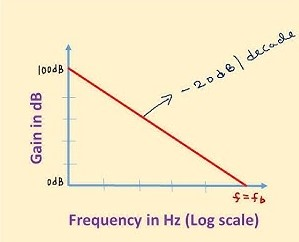
\includegraphics[width=0.5\textwidth]{idealIntegrator.jpg}
    \caption{Ideal Integrator}
\end{figure}

by adding resistance in parallel with cap we prevent
high loop gain at low frequencies

\begin{figure}[h] % 'h' indicates to place the figure here
    \centering
    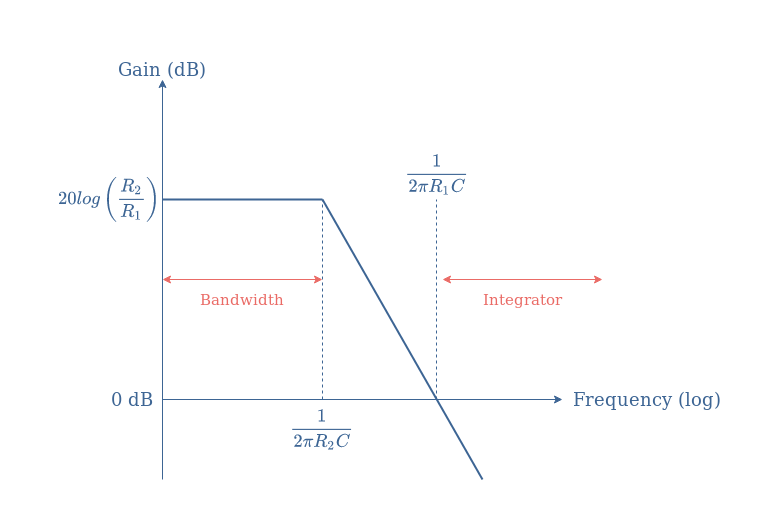
\includegraphics[width=0.4\textwidth]{practical.jpg}
    \caption{Practical Circuit}
\end{figure}


\[
    {R_{comp}}=\frac{R_f . R_{in}}{R_f + R_{in} } \qquad F_L =\frac{1}{2\pi R_f C_f} \qquad F_o =\frac{1}{2\pi R_1 C_f} 
\]

we add compensated resistance at non inverting terminal to limit  bias current
\end{document}
